\graphicspath{{1completeness/asy/}}

\title{Math 140A - Notes}
\author{Neil Donaldson}
\date{\today}
\maketitle

\thispagestyle{empty}


\section*{Introduction}

Analysis is one of the major sub-disciplines of mathematics, being concerned with continuous functions, limits, calculus and accurate approximations.
\smallbreak

Analytic ideas date back over 2000 years. For instance, Archimedes (c.\,287--212\,\BC) used limit-type approaches to approximate the circumference of a circle and compute the area under a parabola.\footnote{Archimedes' circle calculation is reminiscent of the Riemann sum approach to integration, whereas his parabolic area method required the evaluation of the infinite series $\sum_{n=0}^\infty \frac 1{4^n}=\frac 43$.}
The philosophical objections to such calculations are just as old: how can it make sense to sum up infinitely many infinitesimally small quantities? This was part of a deeper debate among the ancient Greeks: is the matter comprising the natural world \emph{atomic} (consisting of minute, discrete, indivisible pieces) or \emph{continuous} (arbitrarily and infinitesimally divisible). Several of Zeno's famous paradoxes (5\th\,C.{}\BC) grapple with these difficulties: \emph{Achilles and the Tortoise} essentially argues that the infinite series $\sum\limits_{n=1}^\infty \frac 1{2^n}=\frac 12+\frac 14+\frac 18+\frac 1{16}+\cdots$ is meaningless.
\begin{center}
	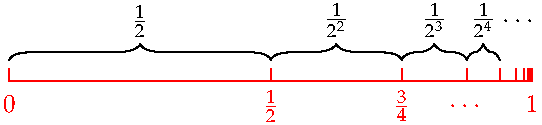
\includegraphics{zeno-jump}
\end{center}
As we'll see, with modern definitions it makes sense for this sum to evaluate to 1.
\smallbreak

The work of Newton and Leibniz in the late 1600s allowed the easy application of calculus to many important problems in the sciences, but without properly addressing the ancient philosophical challenges. The logical development of calculus necessitated by this became the triumph of 18\th--19\th{} century mathematics. The critical notions of limit and continuity only became rigorous in the early 1800s, courtesy of Bolzano, Cauchy and Weierstrass (amongst others), with another 50 years before Riemann provided a thorough description of the definite integral.
\medbreak

The Math 140A/B sequence introduces analysis by focusing on these ideas. In this course we primarily consider sequences, limits, continuity and infinite series. Power series, differentiation and integration are the focus of 140B. We start, however, with something even more basic: to numerically measure continuous quantities, we need to familiarize ourselves with the \emph{real numbers.} Since a concrete description is quite difficult, we build up to it using first the natural numbers and then the rationals\ldots

\goodbreak

\section[The Set N of Natural Numbers]{The Set $\N$ of Natural Numbers}\label{sec:natural}

You've been using the natural numbers $\N=\{1,2,3,4,5,\ldots\}$ since you learned to count. In mathematics, these must be axiomatically described. Here is one approach, known as \emph{Peano's Axioms.}%While reading them, think of the challenge of getting here: what is the essential nature of the natural numbers and what distinguishes them from other sets such as the rationals and reals?

\begin{axioms}{}{Peano}
	The natural numbers are a set $\N$ satisfying the following properties:
	\begin{enumerate}
	  \item (Non-emptiness)\lstsp $\N$ is non-empty.
		\item (Successor function)\lstsp There exists a function $f:\N\to\N$. This function is usually denoted `$+1$' so that we may write,
		\[n\in\N\implies n+1\in\N\]
		\item (Initial element)\lstsp $f$ is \emph{not surjective.} Otherwise said, there exists an element $1\not\in\operatorname{range}f$ which is not the successor of any element.\footnotemark
		\item (Unique predecessor/order)\lstsp $f$ is \emph{injective.} If $m$ and $n$ have the same successor, then $m=n$. 
		\item (Induction)\lstsp Suppose $A\subseteq\N$ is a subset satisfying
		\begin{enumerate}
		  \item $1\in A$
		  \item $n\in A\implies n+1\in A$.
		\end{enumerate}
		Then $A=\N$.
	\end{enumerate}
\end{axioms}

\footnotetext{It is purely convention to denote the first natural number by 1; we could use 0, $x$, $\alpha$, or any symbol you wish!}

Axioms 1--4 are relatively straightforward, the natural numbers are defined by repeatedly adding 1 to the initial element; for instance
\[3:=f\bigl(f(1)\bigr)=(1+1)+1\]
To see why Axiom 5 is so-named, compare an easy example with a standard induction argument.

\begin{example}{}{}
	Prove that $7^n-4^n$ is divisible by 3 for all $n\in\N$.
	\smallbreak
	Let $A$ be the set of natural numbers for which $7^n-4^n$ is divisible by 3. It is required to prove that $A=\N$.
	\begin{enumeratea}
	  \item If $n=1$, then $7^1-4^1=3$, whence $1\in A$.
	  \item Suppose $n\in A$. Then $7^n-4^n=3\lambda$ for some $\lambda\in\N$. But then
		\begin{align*}
		7^{n+1}-4^{n+1}&=7\cdot 7^n-4^{n+1}=7(3\lambda+4^n)-4^{n+1}=3\cdot 7\lambda+(7-4)\cdot 4^n\\
		&=3\bigl(7\lambda+4^n\bigr)
		\end{align*}
	is divisible by 3. It follows that $n+1\in A$.
	\end{enumeratea}
	Appealing to axiom 5, we see that $A=\N$, hence result.\smallbreak
	The two arguments are precisely the familiar \emph{base case} and \emph{induction step}.
\end{example}



% Induction often written in terms of `propositions': I.e. $P_n$ is statement ``$n\in A$''
% 
% \begin{example}
% Prove that $\ln n<n$ for all $n\in \N$
% \begin{itemize}
%   \item Let $P_n$ be the statement: ``$\ln n<n$''
%   \item Clearly $P_1$ is true: $0=\ln 1<1$
%   \item Assume $P_n$ is true for some $n$. Then consider the function $f(x)=\ln x$. Since $f'(x)=\frac 1x$, the MVT says
%   \[\ln(n+1)-\ln n=\frac{\ln(n+1)-\ln n}{n+1-n}=\frac 1x\]
%   for some $x\in(n,n+1)$. In particular
%   \[\ln(n+1)<\ln n+\frac 1n\le \ln n+1\]
%   But $P_n$ says $\ln n<n$, whence $\ln(n+1)<n+1$, so $P_{n+1}$ is true.
% \end{itemize}
% \end{example}
% 
% Recall: Induction can start at any integer and be \emph{strong}
% 
% \begin{example}
% The Fibonacci numbers satisfy $a_1=1,a_2=1$, $a_{n+2}=a_{n+1}+a_n$ for all $n\in\N$. Prove that $a_n\ge n$ for all $n\ge 5$.
% \begin{itemize}
%   \item Let $P_n$ be the statement: ``$a_n\ge n$''
%   \item Clearly $P_5$ is true: $a_5=5$
%   \item And $P_6$: $a_6=8\ge 6$
%   \item Assume $P_n$, $P_{n+1}$ true for some $n\ge 5$. Then
%   \[a_{n+2}=a_n+a_{n+1}\ge n+n+1=2n+1\]
%   However, $2n+1-(n+2)=n-1>0$ for $n\ge 5$, whence $a_{n+2}>n+2$ and $P_{n+2}$ is true.
% \end{itemize}
% \end{example}
% 
% \Endlec 1

\boldinline{What about the integers?}

It should be clear that the integers satisfy axioms 1, 2 and 4, but not 3 and 5. For instance:
\begin{itemize}
  \item[$\not\!3$.] The function $f:\Z\to\Z:n\mapsto n+1$ is surjective (indeed bijective/invertible). The number 1 is the successor of 0.  
  %\item[$\not\!5$.] See Exercise \ref{exs:1notinduction}.
\end{itemize}

We can reverse this observation to provide an explicit construction of the integers from the natural numbers. Simply extend the function $f$ so that \emph{every} element has a unique predecessor: 0 is the unique predecessor of 1, $-1$ the unique predecessor of 0, etc. In essence we are forcing $f(n)=n+1$ to be bijective!
\goodbreak

\begin{exercisessec}{}{}
Most of these exercises are to refresh your memory of mathematical induction. You can use either the language of Peano's axiom 5, or the (likely) more familiar base-case/induction-step formulation.
%\exstart 

\begin{enumerate}%\setcounter{enumi}{1}
  \item%[1.]
  Prove that $1^2+2^2+\cdots+n^2=\frac 16n(n+1)(2n+1)$ for all natural numbers $n$.
  
  \item%[2.]
  Prove that $3+11+\cdots+(8n-5)=4n^2-n$ for all $n\in\N$.

  \item%[4.]
  \begin{enumeratea}
  	\item  Guess a formula for $1+3+\cdots+(2n-1)$ by evaluating the sum for $n=1,2,3$, and 4.\par
  	(\emph{For $n=1$ the sum is simply 1})
  
  	\item Prove your formula using mathematical induction.
  \end{enumeratea}
  
  \item%[6.]
  Prove that $11^n-4^n$ is divisible by 7 for all $n\in\N$.
  
  \item%[8.]
  The principle of mathematical induction can be extended as follows. A list $P_m,P_{m+1},\ldots$ of propositions is true provided (i) $P_m$ is true, (ii) $P_{n+1}$ is true whenever $P_n$ is true and $n\ge m$.
  \begin{enumeratea}
  \item Prove that $n^2>n+1$ for all integers $n\ge 2$.
  \item Prove that $n!>n^2$ for all integers $n\ge 4$.\par
  	(\emph{Recall that $n!=n(n-1)\cdots 2\cdot 1$})
  \end{enumeratea}
  
  \item%[10.]
  Prove $(2n+1)+(2n+3)+(2n+5)+\cdots+(4n-1)=3n^2$ for all $n\in\N$.
  
  \item%[11.]
  For each $n\in\N$, let $P_n$ denote the assertion ``$n^2+5n+1$ is an even integer''.
  \begin{enumeratea}
  \item Prove that $P_{n+1}$ is true whenever $P_n$ is true.
  \item For which $n$ is $P_n$ actually true? What is the moral of this exercise?
  \end{enumeratea}
  
%   \item%[12.] 
%For $n\in\N$, let $n!$ denote the factorial function. Also let $0!=1$ and define the binomial coefficient
%   \[\binom nk=\frac{n!}{k!(n-k)!}\quad\text{for}\quad\ k=0,1,\ldots,n\]
%   The \emph{binomial theorem} asserts that, for all $n\in\N$,
%   \[(a+b)^n=\binom n0a^n+\binom n1a^{n-1}b+\binom n2a^{n-2}b^2+\cdots+\binom n{n-1}ab^{n-1}+\binom nnb^n=\sum_{k=0}^n\binom nka^{n-k}b^k\]
%   \begin{enumeratea}
%   \item Verify the binomial theorem for $n=1,2$, and 3.
%   \item Show that $\binom nk+\binom n{k-1}=\binom{n+1}k$ for $k=1,2,\ldots,n$.
%   \item Prove the binomial theorem by mathematical induction.
%   \end{enumeratea}


  \item Show that Peano's induction axiom is \emph{false} for the set of integers $\Z$  by exhibiting a \emph{proper subset} $A\subset\Z$ which satisfies conditions (a) and (b).
  
  \item Consider $\Z_3=\{0,1,2\}$ under addition modulo 3. That is,
  \[0+1=1,\quad 1+1=2,\quad 2+1=0\]
  Which of Peano's axioms are satisfied?
\end{enumerate}
\end{exercisessec}

\clearpage




\section[The Set Q of Rational Numbers]{The Set $\Q$ of Rational Numbers}\label{sec:Q}

There are several ways to define the rational numbers from the integers. For instance, we could consider the set of relatively prime ordered pairs
\[\Q=\bigl\{(p,q):p\in\Z,\ q\in\N,\, \gcd(p,q)=1\bigr\}\subseteq\Z\times\N\]
Things are more familiar once we write $\frac pq$ instead of $(p,q)$ and adopt the convention that $\frac{\lambda p}{\lambda q}=\frac pq$ for any non-zero $\lambda\in\Z$. It is easy to define the usual operations ($+,\cdot$, etc.) consistently with those for the integers (Exercise \ref{exs:ratnumber+x}).
\smallbreak

An alternative approach involves equations. Each \emph{linear equation} $qx-p=0$ where $p,q\in\Z$ and $q\neq 0$ corresponds to a rational number! For example
\[13x+27=0\leftrightsquigarrow x=-\frac{27}{13}\]
Of course $26x+54=0$ \emph{also} corresponds to the same rational number!
\smallbreak

% \begin{lemm}
% $\sqrt 2\notin\Q$
% \end{lemm}
% 
% \begin{proof}
% Suppose $\sqrt 2\in\Q$. Then $\sqrt 2=\frac pq$ (assume in lowest terms). Then $q^2=2p^2$ is even. So $q=2k$. Then $2k^2=p^2$ is even. So $p=2l$. Contradiction!
% \end{proof}

%\subsubsection*{Irrational numbers and the rational roots theorem}

Extending this process, we might consider higher degree polynomials.

\begin{defn}{}{}
	A number $x$ is \emph{algebraic} if it satisfies an equation of the form\footnotemark
	\[a_nx^n+a_{n-1}x^{n-1}+\cdots+a_1x+a_0=0\tag*{$(\ast)$}\]
	for some integers $a_0,\ldots,a_n$.
\end{defn}

\footnotetext{You should be alarmed by this! We have given up on \emph{constructing} new numbers and instead are simply \emph{describing} their properties. No matter, a construction of the real numbers will come later.}

\begin{examples}{}{}
	\exstart $\sqrt 2$ is algebraic since it satisfies the equation $x^2-2=0$.

	\begin{enumerate}\setcounter{enumi}{1}
	  \item $x=\sqrt[5]{7+\sqrt 3}$ is also algebraic:
	  \[x^5-7=\sqrt 3\implies (x^5-7)^2=3\implies x^{10}-14x^5+46=0\]
	\end{enumerate}
\end{examples}


The next result is helpful for deciding whether a given number is rational and can assist with factorizing polynomials.

\begin{thm}{Rational Roots}{}
	Suppose that $a_0,\ldots,a_n\in\Z$ and that $x\in\Q$ satisfies $(\ast)$. If $x=\frac pq$ in lowest terms, then $p\mid a_0$ and $q\mid a_n$.
\end{thm}

\begin{proof}
	Since $x$ satisfies the polynomial, we see that
	\[a_n\left(\frac pq\right)^n+\cdots+a_1\left(\frac pq\right)+a_0=0\implies a_np^n+a_{n-1}p^{n-1}q+\cdots+a_1pq^{n-1}+a_0q^n=0\]
	All terms except the last contain a factor of $p$, whence $p\mid a_0q^n$. Since $\gcd(p,q)=1$ it follows that $p\mid a_0$. The result for $q$ is almost identical.
\end{proof}

\goodbreak

\begin{examples}{}{}
	\exstart We show that $\sqrt 2$ is irrational.\footnotemark{} Plainly $x=\sqrt 2$ satisfies the polynomial equation $x^2-2=0$. If $\sqrt 2=\frac pq$ were rational in lowest terms, then the rational roots theorem forces
	  \[p\mid 2\quad\text{and}\quad q\mid 1\implies \sqrt 2\in\{\pm 1,\pm 2\}\]
	  Since none of the numbers $\pm 1,\pm 2$ satisfy $x^2-2=0$, we have a contradiction.

	\begin{enumerate}\setcounter{enumi}{1}
		\item $(\sqrt 3-1)^{1/3}$ is irrational. It satisfies $(x^3+1)^2=3$, from which
		\[x^6+2x^3-2=0\]
		By the theorem, if $x=\frac pq$ were rational then $p\mid 2$ and $q\mid 1$, whence $x=\pm 1,\pm 2$, none of which satisfies $(x^3+1)^2=3$.
		\item $\left(\frac{4+\sqrt 3}{5}\right)^{1/2}$ is irrational. It satisfies $5x^2-4=\sqrt 3$, from which
		\[25x^4-40x^2+13=0\]
		If $x=\frac pq$ were rational, then $p\mid 13$ and $q\mid 25$. There are twelve possibilities in all:
		\[x=\pm 1,\pm 13,\pm\frac 15,\pm\frac{13}5,\pm\frac 1{25},\pm\frac{13}{25}\]
		It is tedious to check all cases, but none satisfy the required polynomial.
		\par
		With this example it is easier to bypass the theorem entirely: if $x\in\Q$ then $\sqrt 3=5x^2-4$ would also be rational!
		
		\item We factorize the polynomial $3x^3+x^2+x-2=0$. By the rational roots theorem, if $x=\frac pq$ is a rational root, then $p\mid 2$ and $q\mid 3$ which gives several possibilities:
		\[x\in\left\{\pm 1,\pm 2,\pm\frac 13,\pm\frac 23\right\}\]
		It doesn't take long to try these and observe that $x=\frac 23$ is the only rational solution. The polynomial has a factor of $3x-2$ which we can extract by long division to obtain
		\[3x^3+x^2+x-2=(3x-2)(x^2+x+1)\]
		The quadratic has no real roots: absent complex numbers, the factorization is complete.
	\end{enumerate}
\end{examples}

\footnotetext{Compare this to the standard proof of the irrationality of $\sqrt 2$ as seen in a previous course. Note how easy it is to extend our approach to $\sqrt 3$, $\sqrt{29}$, $\sqrt[3]{2}$, $\sqrt[5]{8}$, etc.}



It is far from clear that there exist non-algebraic (or \emph{transcendental}) numbers, of which $e$ and $\pi$ are the most famous examples. These satisfy no polynomial equation with integer coefficients, though demonstrating this is tricky.
% 
% We finish with a nice corollary which allows us to decide precisely which square-roots of integers are rational.
% 
% \begin{cor}{}{}
% Let $n\in\N$. Then $\sqrt n$ is rational if and only if it is an integer.
% \end{cor}
% 
% Otherwise said, $\sqrt n$ is irrational unless $n$ is a perfect square.
% 
% \begin{proof}
% $\sqrt n$ satisfies $x^2-n=0$. If $\sqrt n=\frac pq$ with $\gcd(p,q)=1$, the rational roots theorem implies that $q\mid 1$. It follows that $x=\sqrt n=p$ is itself an integer.
% \end{proof}


\begin{exercisessec}{}
	\exstart Describe all the linear equations which correspond to the rational number $\frac{101}{29}$.
	
	\begin{enumerate}\setcounter{enumi}{1}
	  \item %[1.]
	  Show that $\sqrt 3$, $\sqrt 5$ and $\sqrt{24}$ are not rational numbers.\par
	  (\emph{Hint: what are the relevant polynomials?})
	  
	  \item %[2.]* 
	  Show that $2^{1/3}$ and $13^{1/4}$ are not rational numbers.
	
	  \item%[3.]
	  Show that $(2+\sqrt 2)^{1/2}$ is not rational.
	  
	%   \item%[4.]* 
	%   Show that $(5-\sqrt 3)^{1/3}$ is not rational.
	  
	  \item%[5.] 
	  Show that $(3+\sqrt 2)^{2/3}$ is not rational.
	  
	  \item%[6.]* 
	  Explain why $4-7b^2$ must be rational if $b$ is rational.
	  
	  \item\label{exs:ratnumber+x} Given rational numbers $(p,q)$ and $(r,s)$ as ordered pairs, what are the rational numbers $(p,q)+(r,s)$ and $(p,q)\cdot(r,s)$?\par
	  (\emph{Hint: what is $\frac pq+\frac rs$?})
	  
	  \item Let $n\in\N$. Use the rational roots theorem to prove that $\sqrt n$ is rational if and only if it is an \emph{integer.}
	\end{enumerate}
\end{exercisessec}

\clearpage



\section{Ordered Fields}

Thus far, we have formally constructed the natural numbers and used them to (loosely) build the integers and rational numbers. It is a significantly greater challenge to \emph{construct} the real numbers. We start by thinking about ordered fields, of which both $\Q$ and $\R$ are examples.

\begin{axioms}{}{field}
	A \emph{field} $\F$ is a set together with two binary operations $+$ and $\cdot$ which satisfy the following (for all $a,b,c\in\F$),\footnotemark
	\medbreak
	$\def\arraystretch{1.3}
	\begin{array}{|l|l|l|}
	\hline
	&\multicolumn{1}{|c|}{\text{Addition}}
	&
	\multicolumn{1}{c|}{\text{Multiplication}}\\\hline
	\text{Closure}&a+b\in\F &ab\in\F\\\hline
	\text{Associativity}&a+(b+c)=(a+b)+c &a(bc)=(ab)c\\\hline
	\text{Commutativity}&a+b=b+a &ab=ba\\\hline
	\text{Identity}&\exists 0\in\F\text{ such that }a+0=a &\exists 1\in\F \text{ such that }a\cdot 1=a\\\hline
	\text{Inverse}&\exists -a\in\F \text{ such that }a+(-a)=0 &\text{If }a\neq 0,\ \exists a^{-1}\in\F\text{ such that }aa^{-1}=1\\\hline\hline
	\text{Distributivity}&\multicolumn{2}{|l|}{a(b+c)=ab+ac}\\\hline
	\end{array}
	$
	\bigbreak
	% \begin{itemize}
	% 	\item[A0] $a+b\in\F$
	% 	\item[A1] $a+(b+c)=(a+b)+c$
	% 	\item[A2] $a+b=b+a$
	% 	\item[A3] $\exists 0\in\F$ such that $a+0=a$
	% 	\item[A4] $\exists -a\in\F$ such that $a+(-a)=0$
	% 	\item[M0] $ab\in\F$ \ (closure)
	% 	\item[M1] $a(bc)=(ab)c$ \ (associativity)
	% 	\item[M2] $ab=ba$ \ (commutativity)
	% 	\item[M3] $\exists 1\in\F$ such that $a\cdot 1=a$ \ (identity)
	% 	\item[M4] If $a\in\F\setminus\{0\}$, $\exists a^{-1}\in\F$ such that $aa^{-1}=1$ \ (inverse)
	% 	\item[D] $a(b+c)=ab+ac$ \ (distributivity)
	% \end{itemize}
	A field $\F$ is \emph{ordered} if we also have a binary relation $\le$ which satisfies (again for all $a,b,c\in\F$):
	\begin{itemize}%\itemsep0pt
		\item[O1] $a\le b$ or $b\le a$
		\item[O2] $a\le b$ and $b\le a\implies a=b$
		\item[O3] $a\le b$ and $b\le c\implies a\le c$
		\item[O4] $a\le b\implies a+c\le b+c$
		\item[O5] $a\le b$ and $0\le c\implies ac\le bc$
	\end{itemize}
\end{axioms}

\footnotetext{We write multiplication $\cdot$ as juxtaposition unless it is helpful for clarity. We also use the common shorthand $a^2=a\cdot a$. If you know some abstract algebra:
\begin{itemize}%\setlength{\itemsep}{0pt}
  \item The addition axioms say that $\bigl(\F,+\bigr)$ is an abelian group.
  \item The multiplication axioms say that $\bigl(\F\setminus\{0\},\cdot\bigr)$ is an abelian group.
  \item The distributive axiom describes how addition and multiplication interact.
\end{itemize}}

For an ordered field, the symbol $<$ is used in the usual way: $x<y\iff x\le y$ and $x\neq y$.
\smallbreak

% \begin{axioms}{Ordered Field}{ord}
% An \emph{ordered field} is a field $\F$ together with a binary relation $\le$ such that, for all $a,b,c\in\F$,
% \begin{itemize}
% 	\item[O1] $a\le b$ or $b\le a$
% 	\item[O2] $a\le b$ and $b\le a\implies a=b$
% 	\item[O3] $a\le b$ and $b\le c\implies a\le c$
% 	\item[O4] $a\le b\implies a+c\le b+c$
% 	\item[O5] $a\le b$ and $0\le c\implies ac\le bc$
% \end{itemize}
% \end{axioms}

As with Peano's axioms for the natural numbers, these are not worth memorizing. Instead you should quickly check that you believe all of them for your current understanding of the real numbers; you can't \emph{prove} anything since the real numbers haven't yet been defined!
\smallbreak


\begin{example}{}{qordered}
	It is worth considering the rational numbers in a little more detail. Recall (Section \ref{sec:Q}) how $\Q$ may be defined as a set of ordered pairs $\frac pq\leftrightsquigarrow(p,q)\in\Z\times \N$. It moreover inherits a natural ordering from $\Z$ and $\N$:
	\[\frac pq\le\frac rs\iff ps\le qr \tag{remember that $q,s>0$}\]
  It is now possible, though tedious, to \emph{prove} that each of the axioms of an ordered field holds for $\Q$, using only basic facts about multiplication, addition and ordering \emph{within the integers.} For instance,
  \begin{itemize}
% 		\item[M2] Given $a=\frac pq$ and $b=\frac st$ rational, we have
% 		\[ab=\frac{ps}{qt}=\frac{sp}{qt}=ba\]
% 		since multiplication of integers is commutative.
		\item[O3] Suppose $a\le b$ and $b\le c$. Write $a=\frac pq$, $b=\frac rs$ and $c=\frac tu$ where all three denominators are positive. By assumption,
		\begin{align*}
			ps\le qr\ \text{ and }\ ru\le st &\implies psu\le qru\le qst\implies pu\le qt\\
			&\implies a=\frac pq\le\frac tu= c
		\end{align*}
	\end{itemize}
\end{example}

\boldsubsubsection{Basic Results about ordered fields}

As with the axioms of an ordered field, it is not worth \emph{memorizing} these.

\begin{thm}{}{orderedfprops}
	Let $\F$ be a ordered field with at least two elements $0\neq 1$. Then:\smallbreak
	\def\arraystretch{1.4}
	\begin{tabular}{rl@{\qquad}rl}
	  1.&$a+c=b+c\implies a=b$ &2.&$a\cdot 0=0$\\
	  3.&$(-a)b=-(ab)$&4.&$(-a)(-b)=ab$\\
	  5.&$ac=bc$ and $c\neq 0\implies a=b$ &6.&$ab=0\implies a=0$ or $b=0$\\
	  7.&$a\le b\implies -b\le -a$&8.&$a\le b$ and $c\le 0\implies bc\le ac$\\
	  9.&$0\le a$ and $0\le b\implies 0\le ab$&10.&$0\le a^2$\\
	  11.&$0<1$&12.&$0<a\implies 0<a^{-1}$\\
	  13.&$0<a<b\implies 0<b^{-1}<a^{-1}$&&
	\end{tabular}
% \begin{enumeratea}\itemsep0pt
%   \item $a+c=b+c\implies a=b$
%   \item $a\cdot 0=0$
%   \item $(-a)b=-(ab)$
%   \item $(-a)(-b)=ab$
%   \item $ac=bc$ and $c\neq 0\implies a=b$
%   \item $ab=0\implies a=0$ or $b=0$
%   \item $a\le b\implies -b\le -a$
%   \item $a\le b$ and $c\le 0\implies bc\le ac$
%   \item $0\le a$ and $0\le b\implies 0\le ab$
%   \item $0\le a^2$
%   \item $0<1$
%   \item $0<a\implies 0<a^{-1}$
%   \item $0<a<b\implies 0<b^{-1}<a^{-1}$
% \end{enumeratea}
\end{thm}

All of these statements should be intuitive for the fields $\Q$ and $\R$. Try \emph{proving} a few using only the axioms; they are easiest done in the order presented. For instance, part 2 might be proved as follows:
\begin{align*}
&a\cdot 0+0=a\cdot 0=a\cdot(0+0)=a\cdot 0+a\cdot 0 \tag{additive identity/distibutive axioms}\\
\implies &0=a\cdot 0 \tag{part 1}
\end{align*}

We finish with one final useful ingredient.

\begin{defn}{}{}
	If $\F$ is an ordered field, then the \emph{absolute value} of $a\in\F$ is
	\[\nm a:=\begin{cases}
	a&\text{if }a\ge 0\\
	-a&\text{if }a<0
	\end{cases}\]
\end{defn}

\begin{thm}{}{}
	In any ordered field:
	\begin{enumerate}
	\item $\nm a\ge 0$
	\item $\nm{ab}=\nm a\cdot \nm b$
	\item $\nm{a+b}\le \nm a+\nm b$ \lstsp ($\triangle$-inequality)%\footnote{The name comes from the corresponding result for \emph{vectors} $\nm{\va+\vb}\le \nm{\va}+\nm{\vb}$. If a triangle has two edges described vectors $\va$ and $\vb$ then the third edge $\va+\vb$ has length no more than the sum of the other two sides.})
	\end{enumerate}
\end{thm}

All three parts are immediate if you consider the $\pm$-cases separately for $a,b$.

% \begin{proof}
% For (a) and (b) just check the $\pm$ cases. For part (c), observe that
% \[-\nm a-\nm b\le a+b\le \nm a+\nm b\]
% which is obvious by thinking about the $\pm$ cases. The result is immediate.
% \end{proof}

% Version not really about triangles: instead  which is proved differently (using Cauchy--Schwarz)
% 
% \Endlec 3


\begin{exercisessec}{}{}
	\exstart %[1.]
	Which of the axioms of an ordered field fail for $\N$? For $\Z$?
	
	\begin{enumerate}\setcounter{enumi}{1}
	  \item%[4.]
	  Prove parts 11 and 13 of Theorem \ref{thm:orderedfprops}.\par%from class ((v) and (vii) of Theorem 3.2 in the book).
	  (\emph{Remember you can use any of the parts that come before\ldots})
	
	  \item%[6.]
	  \begin{enumeratea}
	  	\item Prove that $\nm{a+b+c}\le \nm a+\nm b+\nm c$ for all $a,b,c\in\R$.\par
	  	(\emph{Hint: Apply the triangle inequality twice. Don't consider eight separate cases!})
	  	\item Use induction to prove
	  	\[\nm{a_1+a_2+\cdots+a_n}\le\nm{a_1}+\nm{a_2}+\cdots+\nm{a_n}\]
	  	for any $a_1,\ldots,a_n\in\R$.
	  \end{enumeratea}
	
	  \item%[7.]
	  \begin{enumeratea}
	  	\item Show that $\nm b<a\iff -a<b<a$.
	  	\item Show that $\nm{a-b}<c\iff b-c<a<b+c$
	  	\item Show that $\nm{a-b}\le c\iff b-c\le a\le b+c$
	  \end{enumeratea}
	
	  \item%[8.]*
	  Let $a,b\in\R$. Show that if $a\le b_1$ for every $b_1>b$, then $a\le b$.\par
	  (\emph{Hint: draw a picture if you're stuck. This is a very important example!})
	  
	  \item Following Example \ref{ex:qordered}, prove that $\Q$ satisfies axiom O5.\par
	  (\emph{Hint: if $a=\frac pq$, etc., what is meant by $ac\le bc$?}) 
	  
	  \item (Hard!)\lstsp The complex numbers $\C=\{x+iy:x,y\in\R\}$ form a field. Consider the lexicographic ordering of $\C$ defined by
	  \[x+iy\le p+iq\iff\begin{cases}
	  x<p\text{ or}\\
	  x=p\text{ and }y\le q
	  \end{cases}\]
	  Which of the order axioms O1--O5 are satisfied by the lexicographic ordering?\par
	  (\emph{Don't prove your claims if an axiom is satisfied, but provide a counter-example if not})
	\end{enumerate}
\end{exercisessec}

\clearpage



\section[The Completeness Axiom]{The Completeness Axiom}

While we still haven't provided an explicit \emph{definition} of the real numbers, you should be comfortable with the fact that both $\Q$ and $\R$ are ordered fields. The question remains of how to distinguish them? Perhaps surprisingly, only one additional axiom is required: the \emph{completeness axiom} or \emph{least upper bound principle.} To explain this we first need some terminology.

\begin{defn}{Maxima, Minima \& Boundedness}{}
	Let $S\subseteq\R$ be non-empty.
	\begin{enumerate}
		\item $S$ is \emph{bounded above} if it has an \emph{upper bound} $M$:
		\[\exists M\in\R\text{ such that }\forall s\in S,
		\ s\le M\]
		\item We write $M=\max S$, the \emph{maximum} of $S$, if $M$ is an upper bound for $S$ \emph{and} $M\in S$.
		\item $S$ \emph{bounded below}, a \emph{lower bound} $m$, and the \emph{minimum} $\min S$ are defined similarly.
		\item $S$ is \emph{bounded} if it is bounded above and below. We say that $S$ is \emph{bounded by $M$} if
		\[\forall s\in S,\ \nm s\le M\]
	\end{enumerate}
\end{defn}

\begin{examples}{}{}
	\exstart If $S$ is a finite set, then it is bounded and has both a maximum and a minimum. For instance, $S=\{-3,\pi,12\}$ has $\min S=-3$ and $\max S=12$.
	\begin{enumerate}\setcounter{enumi}{1}
		\item $\N$ has minimum 1, but no maximum. $\Z$ and $\Q$ have neither: both are \emph{unbounded.}
		\item The interval $S=[0,3)=\{x\in\R:0\le x<3\}$ is bounded, for example by $M=5$, it has minimum 0 and no maximum. While this last is likely intuitive, it worth giving an explicit argument, in this case by contradiction.\par
		Suppose $x=\max S$ exists. It is helpful to draw a picture to get the lay of the land. Since $x\in S$, we've placed $x$ \emph{inside} the interval, away from 3.
		\begin{center}
	  	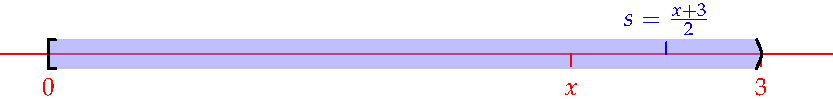
\includegraphics{nomax1}
	  \end{center}
	  The crux of the proof is to observe that there exists $s\in S$ which is \emph{larger} than $x$. The natural choice is the average $s:=\frac 12(x+3)$. Now observe that
	  \[3-s=s-x=\frac 12(3-x)>0\]
	  In particular,
		\begin{itemize}
		  \item $s\in S$ since it is non-negative and $s<3$.
		  \item $s>x$.
		\end{itemize}
		Since $S$ contains an element larger than $x$, it follows that $x$ cannot be the maximum of $S$. In conclusion, $S$ has no maximum.
	\end{enumerate}
\end{examples}

\goodbreak

The following should be immediate: try proving them yourself.

\begin{lemm}{}{}
	\exstart If $M$ is an upper bound for $S$, so is $M+\varepsilon$ for any $\varepsilon\ge 0$.
	\begin{enumerate}\setcounter{enumi}{1}
	  \item If $\max S$ exists, then it is unique.
	  \item A set is bounded if and only if it is bounded above and below. In particular, if $m,M$ are lower/upper bounds, then $S$ is bounded by 
	  \[\forall s\in S,\ \nm s\le\max(\nm m,\nm M)\]
	\end{enumerate}
\end{lemm}


\begin{example}{}{qsqqrt2nomax}
	Before introducing the key axiom, we consider a variation on the previous example. We show that the following set has no maximum:
	\[S=\Q\cap[0,\sqrt 2)=\{x\in \Q:0\le x<\sqrt 2\}\]	
	The approach is similar to before: given a hypothetical maximum $x$, find an element $s\in S$ between $x$ and $\sqrt 2$. The challenge is that we can't simply use the \emph{average} $\frac 12(x+\sqrt 2)$: this isn't rational (\emph{why?}) and so doesn't lie in $S$!\smallbreak
	
	To fix this, we informally invoke sequences: this might seem quite hard at the moment, but will be made rigorous later. The rough idea is to construct a sequence $(s_n)$ of elements of $S$ which increases to $\sqrt 2$. Eventually one of these must be larger than $x$.\smallbreak
	
	Define a sequence of rational numbers $(s_n)$ by $s_n=\frac 1{10^n}\lfloor 10^n\sqrt 2\rfloor$, where $\lfloor\ \ \rfloor$ denotes the \emph{floor function}.\footnotemark{} The sequence simply recovers the first $n$ decimal places of $\sqrt 2$:
	\[s_0=1,\quad s_1=1.4=\frac{14}{10},\quad s_2=1.41=\frac{141}{100},\quad s_3=1.414=\frac{1414}{1000},\quad\ldots\]
	and has the following properties:
	\begin{itemize}
	  \item $s_n\in S$ since any truncating decimal is rational and certainly $0\le s_n<\sqrt 2$.
	  \item $\sqrt 2-s_n< 10^{-n}$ follows since $10^n\sqrt 2-\lfloor 10^n\sqrt 2\rfloor< 1$.
	\end{itemize}
	Now suppose $x=\max S$ exists. Since $x\in S$, we have $x<\sqrt 2$. Choose $N\in \N$ large enough so that $10^{-N}<\sqrt 2-x$. Then $s_N\in S$ and
	\[\sqrt 2 -s_N<10^{-N}<\sqrt 2-x\implies x<s_N\]
	The hypothetical maximum $x$ is not an upper bound for $S$: contradiction.
	\begin{center}
	  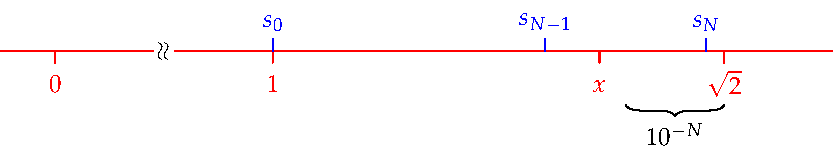
\includegraphics{nomax2}\vspace{-5pt}
	\end{center}
\end{example}

\vspace{-10pt}

\footnotetext{$\lfloor y\rfloor$ is the greatest integer less than or equal to $y$; informally \emph{round down.} For example $\lfloor \pi\rfloor=3$. This approach is a something of a hack: it can be sped up enormously using the upcoming density of $\Q$ in $\R$ (Corollary \ref{cor:qdense}); indeed the Archimedean property on which it depends is necessary for $\lfloor y\rfloor$ to be well-defined.}

\goodbreak


\boldsubsubsection{Suprema and Infima}

We now generalize the idea of maximum and minimum values for bounded sets.

\begin{example}{}{supbasic}
	The interval $[2,5)$ has \emph{least upper bound} 5: among all upper bounds, 5 is the smallest.
\end{example} 

\begin{defn}{}{supinf}
	Let $S\subseteq\R$ be non-empty.
	\begin{enumerate}
	  \item If $S$ is bounded above, its \emph{supremum} $\sup S$ is its \emph{least upper bound.} Otherwise said,
		\begin{enumerate}
	  	\item $\sup S$ is an upper bound:\quad $\forall s\in S,\ s\le \sup S$,
	  	\item $\sup S$ is the least such:\quad if $M$ is an upper bound, then $\sup S\le M$.
		\end{enumerate}
		\item If $S$ is bounded below, its \emph{infimum} $\inf S$ is its \emph{greatest lower bound.} Equivalently,
		\begin{enumerate}
	  	\item $\inf S$ is a lower bound:\quad $\forall s\in S,\ \inf S\le s$,
	  	\item $\inf S$ is the greatest such:\quad if $m$ is a lower bound, then $m\le\inf S$.
		\end{enumerate}
	\end{enumerate}
	
	\begin{center}
		\vspace{-5pt}
		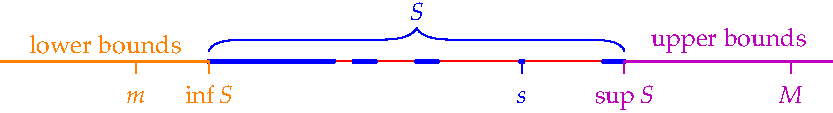
\includegraphics{supinf}
	\end{center}
\end{defn}


\begin{example*}{\ref{ex:supbasic} cont}{}
	We verify the supremum and infimum for $S=[2,5)$; parts (a), (b) are the properties in the above definition.	
	\begin{enumeratea}
		\item Since $s\in S\iff 2\le s<5$, we see that 5 is an upper bound and 2 a lower bound.
		\item Given $x<5$, define\footnotemark{} $s:=\max\{\frac 12(x+5),4\}$. Observe that $x<s<5$ from which $s\in S$ is \emph{larger} than $x$. It follows that $x$ is \emph{not} an upper bound for $S$, and that 5 is the least such.\par
		Similarly, if $y>2$, define $t:=\min\{\frac 12(y+2),4\}$ to see that $t\in S$ is \emph{smaller} than $y$, which cannot therefore be a lower bound for $S$.
% 		\item Suppose some $M>5$ is the least upper bound and consider $\hat M:=\frac 12(M+5)$. Then
% 		 \[5<\hat M<M\tag{check it explicitly!}\]
% 		 so that $\hat M$ is a smaller upper bound for $S$: contradiction.\par
% 		 Similarly, if some $m<2$ were the greatest lower bound, we check that $\hat m:=\frac 12(m+2)$ satisfies $m<\hat m<2$, so that $\hat m$ is a larger lower bound: contradiction.
	\end{enumeratea}
	
	We conclude that $\sup S=5$ and $\inf S=2$.
	
	\begin{center}
		\vspace{-5pt}
		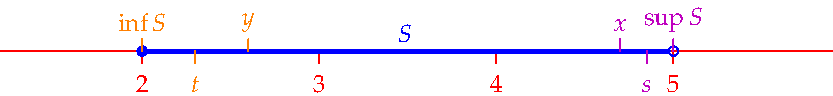
\includegraphics{supinf3}
	\end{center}
\end{example*}

\footnotetext{The number 4 is merely an arbitrary element to make sure $s\in S$ in case $x$ were huge and negative!}

We are assuming something quite important here!

\begin{axiom}{Completeness of $\R$}{comp}
	If $S\subseteq\R$ is non-empty and bounded above, then $\sup S$ exists (and is a real number!).
\end{axiom}

It is this property that distinguishes the real numbers from the rationals.\footnote{\label{fn:syntheticR}If you've studied abstract algebra, then a more rigorous statement should make sense: every ordered field with $0\neq 1$ and which satisfies the completeness axiom is isomorphic to the real numbers.} Note that every bounded set $S$ of \emph{rational} numbers has a supremum; the issue is that $\sup S$ \emph{might not be rational}!

% \begin{aside}{}{}
% 
% {\bf Aside: A Synthetic Construction of $\R$}\qquad We have only observed that completeness is a \emph{property} of $\R$. It is, in fact, the defining difference between $\R$ and $\Q$. Explicitly:
% 
% \begin{thm}{}{}
% Up to relabeling (isomorphism of fields), there is precisely one set $\R$ which satisfies the following properties:
% \begin{itemize}
% \item $\R$ is an ordered field such that $0\neq 1$ (Axioms \ref{axiom:field} and \ref{axiom:ord})
% \item $\R$ has the completeness property (Axiom \ref{axiom:comp})
% \end{itemize}
% \end{thm}
% 
% \def\SSS{\mathbb{S}}
% The proof is too difficult and far too algebraic for us! To unpack things slightly, one must show that if $(\R,0_\R,1_\R,+_\R,\cdot_\R,\le_\R)$ and $(\SSS,0_\SSS,1_\SSS,+_\SSS,\cdot_\SSS,\le_\SSS)$ are two models satisfying the axioms, then there exists an isomorphism $\phi:\R\to\SSS$: that is,
% \begin{enumerate}
%   \item $\phi$ is bijective
%   %\item $\phi(0_\R)=0_\SSS$ and $\phi(1_\R)=1_\SSS$
%   \item $\phi(x+_\R y)=\phi(x)+_\SSS\phi(y)$ and $\phi(x\cdot_\R y)=\phi(x)\cdot_\SSS\phi(y)$ for all $x,y\in\R$
%   \item $x\le_\R y\iff \phi(x)\le_\SSS\phi(y)$
% \end{enumerate}
% 
% This approach will likely only satisfy you if you are addicted to abstract algebra!
% \end{aside}

\goodbreak

\begin{example*}{\ref{ex:qsqqrt2nomax} cont}{}
	The set $S=\Q\cap[0,\sqrt 2)$ has $\sup S=\sqrt 2$. We check conditions (a), (b) in Definition \ref{defn:supinf}.
	\begin{enumeratea}
		\item Certainly $\sqrt 2$ is an upper bound for $S$, since every element is less than $\sqrt 2$.
		\item If $x<\sqrt 2$ is given, then our previous argument says there exists some $s_N\in S$ for which $s_N>x$. Plainly $x$ isn't an upper bound.
	\end{enumeratea}
	In conclusion, $\sqrt 2$ is the smallest upper bound for $S$.
\end{example*}

%\boldinline{A Useful Contrapositive}

Consider the contrapositive of part (b) of Definition \ref{defn:supinf} after replacing $M$ with $x$.

\begin{quote}
	If $x<\sup S$, then $x$ is \emph{not} an upper bound for $S$.
\end{quote}

If we unpack this further, we recover a useful existence result. Indeed this is precisely what we did in both previous examples.

\begin{lemm}{}{contrasup}
	\exstart If $x<\sup S$, then $\exists s\in S$ such that $s>x$.
	\begin{enumerate}\setcounter{enumi}{1}
	  \item If $y>\inf S$, then $\exists t\in S$ such that $t<y$.
	\end{enumerate}

\begin{center}
	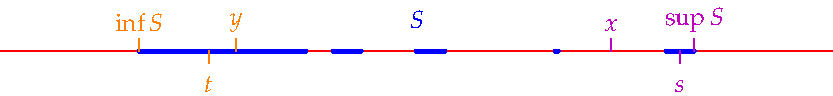
\includegraphics{supinf4}
\end{center}
\end{lemm}

This observation will be used repeatedly, so make sure it is well understood.
%\medbreak

\begin{examples}{}{}
	We state the following without proof or calculation. You should be able to justify all these statements using the definition, or by mirroring the above examples.
	\begin{enumerate}
		\item A bounded set has many possible bounds, but only one supremum or infimum.
		\item If $S$ has a maximum, then $\max S=\sup S$. Similarly $\min S=\inf S$ if a minimum exists.
		%\item The supremum and infimum exist even when a maximum and minimum do not. For instance, $S=(-1,4)$ has $\sup S=4$; the set has no maximum since $\sup S=4\not\in S$. Similarly, $S$ has no minimum and $\inf S=-1\not\in S$.
		\item $S=\Q\cap (\pi,4)$ has $\sup S=4$ and $\inf S=\pi$.
		\item $S=\{\frac 1n:n\in\N\}=\{\ldots,\frac 14,\frac 13,\frac 12,1\}$ has $\sup S=\max S=1$, $\inf S=0$, and no minimum.
		\item $S=\bigcup\limits_{n=1}^\infty [n,n+\frac 12)=[1,1.5)\cup[2,2.5)\cup[3,3.5)\cup\cdots$ has $\inf S=1$. It is not bounded above.
		\item $S=\bigcap\limits_{n=1}^\infty [\frac 1n,1+\frac 1n)$ has $\inf S=1=\sup S$ since $S=\{1\}$.
	\end{enumerate}
\end{examples}

The completeness axiom only asserts the existence of the supremum of a bounded set. By reflecting across zero (see Exercise \ref{exs:infexist}), we obtain the same thing for the infimum.

\begin{thm}{Existence of Infima}{infexist}
If $S\subseteq\R$ non-empty and bounded below, then $\inf S\in\R$ exists.
\end{thm}

\goodbreak

%\begin{proof}
% The picture summarizes the proof:
% \begin{center}
% 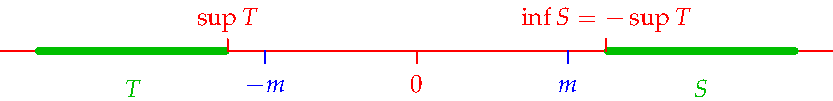
\includegraphics{infexist}
% \end{center}
%\end{proof}




\boldsubsubsection{The Archimedean Property and the Density of the Rationals}

We finish this section by discussing the distribution of the rational numbers among the real numbers. %Indeed, you should think carefully about where exactly we used this property in our discussion on page \pageref{ex:6}.

\begin{thm}{Archimedean Property}{archprop}
If $b>0$ is a real number, then $\exists n\in\N$ such that $n>b$.\par
Equivalently:\footnotemark{} $a,b>0\implies \exists n\in\N$ such that $an>b$.
\end{thm}

\footnotetext{Just replace $b$ with $\frac ba$.}

In this result we assume nothing about $\R$ except that is an ordered field satisfying the completeness axiom and $0\neq 1$. The natural numbers in this context are \emph{defined} as the subset
\[\N=\{1,1+1,1+1+1,\ldots\}\subseteq\R\]
%and Peano's axioms are a \emph{theorem.} %In the next section we'll briefly think about how the Archimidean property is essentially trivial if one has an \emph{explicit} construction of $\R$ built upon $\N$ and $\Q$.

\begin{proof}
Suppose the result were false. Then $\exists b>0$ such that $n\le b$ for all $n\in\N$; that is, $\N$ is bounded above! By completeness, $\sup\N$ exists, and we trivially see that
\[0<1\implies \sup\N<\sup\N+1\implies \sup\N-1<\sup\N\]
By Lemma \ref{lemm:contrasup}, $\exists n\in\N$ such that $n>\sup\N-1$. But then $\sup\N<n+1$ which is clearly a natural number! Thus $\sup\N$ is not an upper bound for $\N$: contradiction.
\end{proof}

The use of completeness is \emph{necessary}: there exist \href{https://en.wikipedia.org/wiki/Non-Archimedean_ordered_field}{non-Archimedean ordered fields!}

\begin{cor}{Density of $\Q$ in $\R$}{qdense}
Between any two real numbers, there exists a rational number.
\end{cor}

The idea is simple: given $a<b$, \textcolor{blue}{stretch} the interval by an integer factor $n$ until it contains an integer $m$, before \textcolor{purple}{dividing} by $n$ to obtain $a<\frac mn<b$. The Archimedean property shows the existence of $m,n$.

\begin{proof}
WLOG suppose $0\le a<b$. The Archimedean property applied to $\frac 1{b-a}>0$ says
\[\exists n\in\N\ \text{such that}\ n>\tfrac 1{b-a}%,\ \text{from which}\ bn>1+an
\]
A second application says $\exists k\in\N$ such that $\textcolor{Green}{k}>\textcolor{blue}{an}$. Now consider
\[J:=\{j\in\N:\textcolor{blue}{an}<\textcolor{Green}{j}\le \textcolor{Green}{k}\}\]
and define $\textcolor{Green}{m}=\min J$: this exists since $J$ is a finite non-empty set of natural numbers.\footnotemark{}
\begin{center}
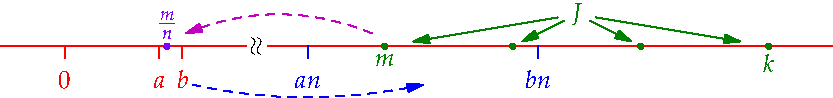
\includegraphics[scale=1]{density}
\end{center}
Clearly $\textcolor{Green}{m}>\textcolor{blue}{an}>m-1$, since $\textcolor{Green}{m}=\min J$. But then $\textcolor{Green}{m}\le an+1<\textcolor{blue}{bn}$. We conclude that
\[\textcolor{blue}{an}<\textcolor{Green}{m}<\textcolor{blue}{bn}\implies a<\textcolor{purple}{\frac mn}<b\tag*{\qedhere}\]
\end{proof}

\footnotetext{This part of the argument is needed because, in this context, we haven't established the well-ordering property of $\N$ (equivalent to Peano's fifth axiom).}

It is immediate that any interval $(a,b)$ now contains \emph{infinitely many} rational numbers.

\goodbreak



\begin{exercisessec}{}{}
	\exstart %(4) parts b,c,f,h,j,l,r,s,v%
	Decide if each set is bounded above and/or below. If it is, \emph{state} its supremum and/or infimum (no working is required).
	\begin{enumerate}\setcounter{enumi}{1}
	  \item[]\begin{enumerate}
	    \item \makebox[130pt][l]{$(0,1)$\hfill (b)} \makebox[170pt][l]{\ $\{2,7\}$\hfill (c)} \ $\{0\}$
	    \setcounter{enumii}{3}
	    \item \makebox[130pt][l]{$\bigcup\limits_{n=1}^\infty[2n,2n+1]$\hfill (e)} \makebox[170pt][l]{\ $\left\{1-\frac 1{3^n}:n\in\N\right\}$\hfill (f)} \ $\{r\in\Q:r^2<2\}$
	    \setcounter{enumii}{6}
	    \item \makebox[130pt][l]{$\bigcup\limits_{n=1}^\infty\left(1-\frac 1n,1+\frac 1n\right)$\hfill (h)} \makebox[170pt][l]{\ $\{\frac 1n:n\in\N$ and $n$ is prime$\}$\hfill (i)} \ $\{\cos(\frac{n\pi}3):n\in\N\}$
  \end{enumerate}

  
  	\item Modelling Example \ref{ex:qsqqrt2nomax}, \emph{sketch} an argument that $S=\Q\cap (\pi,4]$ has no minimum.\par
  	(\emph{Hint: let $s_n$ be $\pi$ rounded \underline{up} to $n$ decimal places})
  
		\item %(6)
		Let $S$ be a non-empty, bounded subset of $\R$.
  	\begin{enumerate}
		  \item Prove that $\inf S\le \sup S$. %(Proof should be short\ldots)
		  \item What can you say about $S$ if $\inf S=\sup S$?
  	\end{enumerate}
  
	  \item %(7) 
	  Let $S$ and $T$ be non-empty subsets of $\R$ with the property that $s\le t$ for all $s\in S$ and $t\in T$.
	  \begin{enumerate}
		  \item Prove that $S$ is bounded above and $T$ bounded below.
		  \item Prove that $\sup S\le \inf T$.
		  \item Give an example of such sets $S,T$ where $S\cap T$ is non-empty.
		  \item Give an example of such sets $S,T$ where $S\cap T$ is empty, and $\sup S=\inf T$.
	  \end{enumerate}
  
	  \item %(9)
	  Prove that if $a>0$ then there exists $n\in\N$ such that $\frac 1n<a<n$.
	  
	
	  \item%(12) 
	  Let $\II=\R\setminus\Q$ be the set of \emph{irrational} numbers. Given real numbers $a<b$, prove that there exists $x\in\II$ such that $a<x<b$.\par
	  (\emph{Hint: First show $\{r+\sqrt 2:r\in\Q\}\subseteq\II$})
  

  	\item %(14)
  	Let $A, B$ be non-empty bounded subsets of $\R$, and let $S$ be the set of all sums
  	\[S:=\{a+b:a\in A,b\in B\}\]
	  \begin{enumerate}
		  \item Prove that $\sup S=\sup A+\sup B$.
		  \item Prove that $\inf S=\inf A+\inf B$.
	  \end{enumerate}
  

  	\item%(16)
  	Show that $\sup\{r\in \Q:r<a\}=a$ for each $a\in\R$.
  
  
  	\item\label{exs:infexist} We prove Theorem \ref{thm:infexist} on the existence of the infimum.\smallbreak
  
	  Let $S\subseteq\R$ be non-empty and let $m$ be a lower bound for $S$. Define $T=\{t\in\R:-t\in S\}$ by \textcolor{red}{reflecting} $S$ across zero.
		\begin{center}
			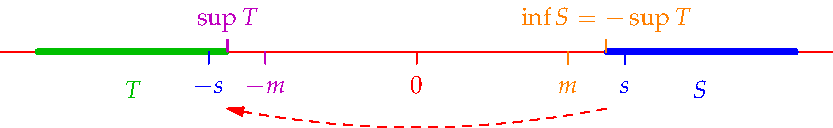
\includegraphics{infexist2}
		\end{center}

		\begin{enumerate}
		  \item Prove that $-m$ is an upper bound for $T$.
			\item By completeness (Axiom \ref{axiom:comp}), $\sup T$ exists. Prove that $\inf S=-\sup T$ by verifying Definition \ref{defn:supinf} parts 2(a) and (b).
		\end{enumerate}
  
	\end{enumerate}
\end{exercisessec}

\clearpage


\section[The Symbols +/- Infinity]{The Symbols $\pm\infty$}

Thus far the only subsets of the real numbers that have a supremum are those which are \emph{non-empty} and \emph{bounded above.} In this very short section, we introduce the $\infty$-symbol to provide all subsets of the real numbers with both a supremum and an infimum.

\begin{defn}{}{}
	Let $S\subseteq\R$ be any subset. If $S$ is bounded above/below, then $\sup S$/$\inf S$ are as in Definition \ref{defn:supinf}. Otherwise:
	\begin{enumerate}
	  \item We write $\sup S=\infty$ if $S$ is \emph{unbounded above}, that is
	  \[\forall x\in \R, \exists s\in S\text{ such that }s>x\]
	  \item We write $\inf S=-\infty$ if $S$ is \emph{unbounded below},
	  \[\forall y\in \R, \exists t\in S\text{ such that }t<y\]
	  \item By convention, $\sup\emptyset:=-\infty$ and $\inf\emptyset:=\infty$, though these will rarely be of use to us.
	\end{enumerate}
\end{defn}

The symbols $\pm\infty$ have \emph{no other meaning} (as yet): in particular, they are \emph{not numbers}! If one is willing to abuse notation and write $x<\infty$ and $y>-\infty$ for any real numbers $x,y$, then the conclusions of Lemma \ref{lemm:contrasup} are precisely statements 1 \& 2 in the above definition!

\begin{examples}{}{}
	\exstart $\sup\R=\sup\Q=\sup\Z=\sup\N=\infty$, since all are unbounded above. We also have $\inf\R=\inf\Q=\inf\Z=-\infty$ (recall that $\inf\N=\min\N=1$).
	\begin{enumerate}\setcounter{enumi}{1}
	  \item If $a<b$, then \emph{any} interval $[a,b]$, $(a,b)$, $[a,b)$ or $(a,b]$ has supremum $b$ and infimum $a$, even if one end is infinite. For example,
		\[S=(7,\infty)=\{x\in\R:x>7\}\]
		has $\sup S=\infty$ and $\inf S=7$.
		\item Let $S=\{x\in\R:x^3-4x<0\}$. With a little factorization, we see that
		\[x^3-4x=x(x-2)(x+2)<0\iff x<-2\text{ or }0<x<2\]
		It follows that $S=(-\infty,-2)\cup(0,2)$, from which $\sup S=2$ and $\inf S=-\infty$.  
	\end{enumerate}
\end{examples}


\begin{exercisessec}{}{}
	\exstart %2
	Give the infimum and supremum of each of the following sets:
	\begin{enumerate}\setcounter{enumi}{1}
  \item[]\begin{enumerate}
    \item \makebox[160pt][l]{$\{x\in\R:x<0\}$ \hfill (b)} \ $\{x\in\R:x^3\le 8\}$
    \setcounter{enumii}{2}
    \item \makebox[160pt][l]{$\{x^2:x\in\R\}$ \hfill (d)} \ $\{x\in\R:x^2<8\}$
  \end{enumerate}
  

  \item%(4)
  Let $S\subseteq\R$ be non-empty, and let $-S=\{-s:s\in S\}$. Prove that $\inf S=-\sup(-S)$.


  \item%(6)
  Let $S,T\subseteq\R$ be non-empty such that $S\subseteq T$. Prove that $\inf T\le \inf S\le \sup S\le\sup T$.
  
  \item If $\sup S<\inf S$, what can you say about $S$?
  
\end{enumerate}
\end{exercisessec}

\clearpage


\section[A Development of R]{A Development of $\R$ (non-examinable)}\label{sec:dedekind}

%In the next section we'll briefly think about how the Archimidean property is essentially trivial if one has an \emph{explicit} construction of $\R$ built upon $\N$ and $\Q$.

The comment in footnote \ref{fn:syntheticR} essentially constitutes a \emph{synthetic} definition of the real numbers: there is essentially just one set with the required properties. It is nice, however, to be able to provide an explicit construction. The following approach uses \emph{Dedekind cuts.}\medbreak

First one defines $\N$, $\Z$ and $\Q$. Use Peano's axioms and proceed as in sections \ref{sec:natural} and \ref{sec:Q}. The operations $+,\cdot$ and $\le$ are defined, first on $\N$ and then for $\Z$ and $\Q$ building on the concepts for the integers.

\begin{defn}{}{dedekind}
A \emph{Dedekind cut} $\alpha^*$ is a non-empty proper subset of $\Q$ with the following properties:
	\begin{enumerate}
  	\item If $r\in\alpha^*$ and $s\in\Q$ with $s<r$, then $s\in\alpha^*$.
  	%\item $\alpha^*$ is bounded above.
  	\item $\alpha^*$ has no maximum.
	\end{enumerate}
	Define $\R$ to be the set of all Dedekind cuts!
\end{defn}

The rough idea is that a real number $\alpha$ corresponds to the Dedekind cut $\alpha^*$ of all \emph{rational numbers less than $\alpha$.} While this is the idea, it doesn't stand up as a \emph{definition} due to circular logic: $\alpha$ cannot be defined in terms of itself! 

\begin{examples}{}{}
	\exstart For any \emph{rational number} $r$, the corresponding \emph{real number} is the Dedekind cut
	\[r^*=\{x\in\Q:x<r\}\]
	\begin{enumerate}\setcounter{enumi}{1}
	  \item[]For instance $4^*=\{x\in\Q:x<4\}$ is the Dedekind cut definition of the  \emph{real number} 4.
	  \item It is a little trickier to explicitly define Dedekind cuts corresponding to irrational numbers, though some are relatively straightforward. For instance the real number $\sqrt 2$ would be the Dedekind cut
		\[\sqrt 2^*=\{x\in\Q:x<0\text{ or }x^2<2\}\]
	\end{enumerate}
\end{examples}

It remains to \emph{prove} that the set of Dedekind cuts satisfies all the axioms of a complete ordered field. The full details are too much for us, so here is a rough overview.
\begin{itemize}
  \item Define the ordering of Dedekind cuts via
	\[\alpha^*\le\beta^*\iff\alpha^*\subseteq\beta^*\]
	One can now prove axioms O1--O3 and that the ordering corresponds to that of $\Q$.
	\item Define addition of cuts via
	\[\alpha^*+\beta^*:=\{a+b:a\in\alpha^*,b\in\beta^*\}\]
	This suffices to prove the addition axioms and O4: a careful definition of $-\alpha^*$ is required.
	\item Multiplication is horrible: if $\alpha^*,\beta^*\ge 0$ then
	\[\alpha^*\beta^*:=\{ab:a\ge 0,a\in \alpha^*,b\ge 0,b\in \beta^*\}\cup\{q\in\Q:q<0\}\]
	which may be carefully extended to cover situations when $\alpha^*$ or $\beta<0$. Once can then prove the multiplication axioms, the final order axiom O5, and the distributive axiom.
	\item The completeness axiom must also be verified, though it comes almost for free! If $A\subseteq\R$ (so that $A$ is a set of Dedekind cuts), then the supremum of $A$ is
	\[\sup A=\bigcup\limits_{\alpha^*\in A}\alpha^*\]
\end{itemize}

An alternative approach to $\R$ using sequences of rational numbers will be given later in the course.


\begin{exercisessec}{}{}
	\exstart %(2) 
  Show that if $\alpha^*,\beta^*$ are Dedekind cuts, then so is
  \[\alpha^*+\beta^*=\{r_1+r_2:r_1\in\alpha^*,r_2\in\beta^*\}\]

	\begin{enumerate}\setcounter{enumi}{1}
	  \item %(4)
	  Let $\alpha^*,\beta^*$ be Dedekind cuts and define the `product':
	  \[\alpha^*\cdot\beta^*=\{r_1r_2:r_1\in\alpha^*,r_2\in\beta^*\}\]
	  \begin{enumeratea}
	  \item Calculate some `products' using the cuts $0^*,1^*$ and $(-1)^*$.
	  \item Discuss why this definition of `product' is unsatisfactory for defining multiplication in $\R$.
	  \end{enumeratea}
	  
	  \item We verify the Archimedean property (Theorem \ref{thm:archprop}) using the Dedekind cut definition of $\R$ (it is somewhat easier since the unboundedness of $\N$ and $\Q$ are baked in).
	  \begin{enumerate}
	    \item Explain why every cut $\beta^*$ is bounded above by some rational number.\par
	    (\emph{Hint: if $\beta^*$ satisfies Definition \ref{defn:dedekind} parts 1 \& 2 but is unbounded above, then what is it?})
	    \item If $\beta^*>0^*$ is a positive cut bounded above by $\frac pq$ with $p,q\in\N$, show that $n:=p+1$ corresponds to a cut for which $n^*>\beta^*$.
		\end{enumerate}
	\end{enumerate}
\end{exercisessec}